\newpage
\section{球函数}
\subsection{Legendre方程}
\label{LegendreFunction}
将Laplace方程$\nabla^2u(r,\theta,\phi)=0$在球坐标系下分离变量(见\nameref{Spherical Harmonics}),将会得到以下连带Legendre方程:
$$
\boxed{\frac{1}{\sin\theta}\frac{d}{d\theta}\left(\sin\theta\frac{d\Theta}{d\theta}\right)+\left[\lambda-\frac{m^2}{\sin^2\theta}\right]\Theta=0}
$$

其中,$m=0,1,2,\dots$

变量代换$x=\cos\theta(-1\le x\le1);\quad y=\Theta$

$$\frac{d}{dx}\left[(1-x^2)\frac{dy}{dx}\right]+\left(\lambda-\frac{m^2}{1-x^2}\right)y=0$$


$$\boxed{(1-x^2)y''-2xy'+\left(\lambda-\frac{m^2}{1-x^2}\right)y=0}$$

$m=0$:Legendre方程
$$
\boxed{(1-x^2)y''-2xy'+\lambda y=0}
$$

\textbf{本征值:}$\lambda_l=l(l+1)\quad(l=0,1,2,...)$(推导见\nameref{LegendreEigenValue});

\textbf{本征函数:} $y_l(x)=\mathrm{P}_l(x)$称为\textbf{Legendre多项式}


\begin{figure}[H]
    \centering 
    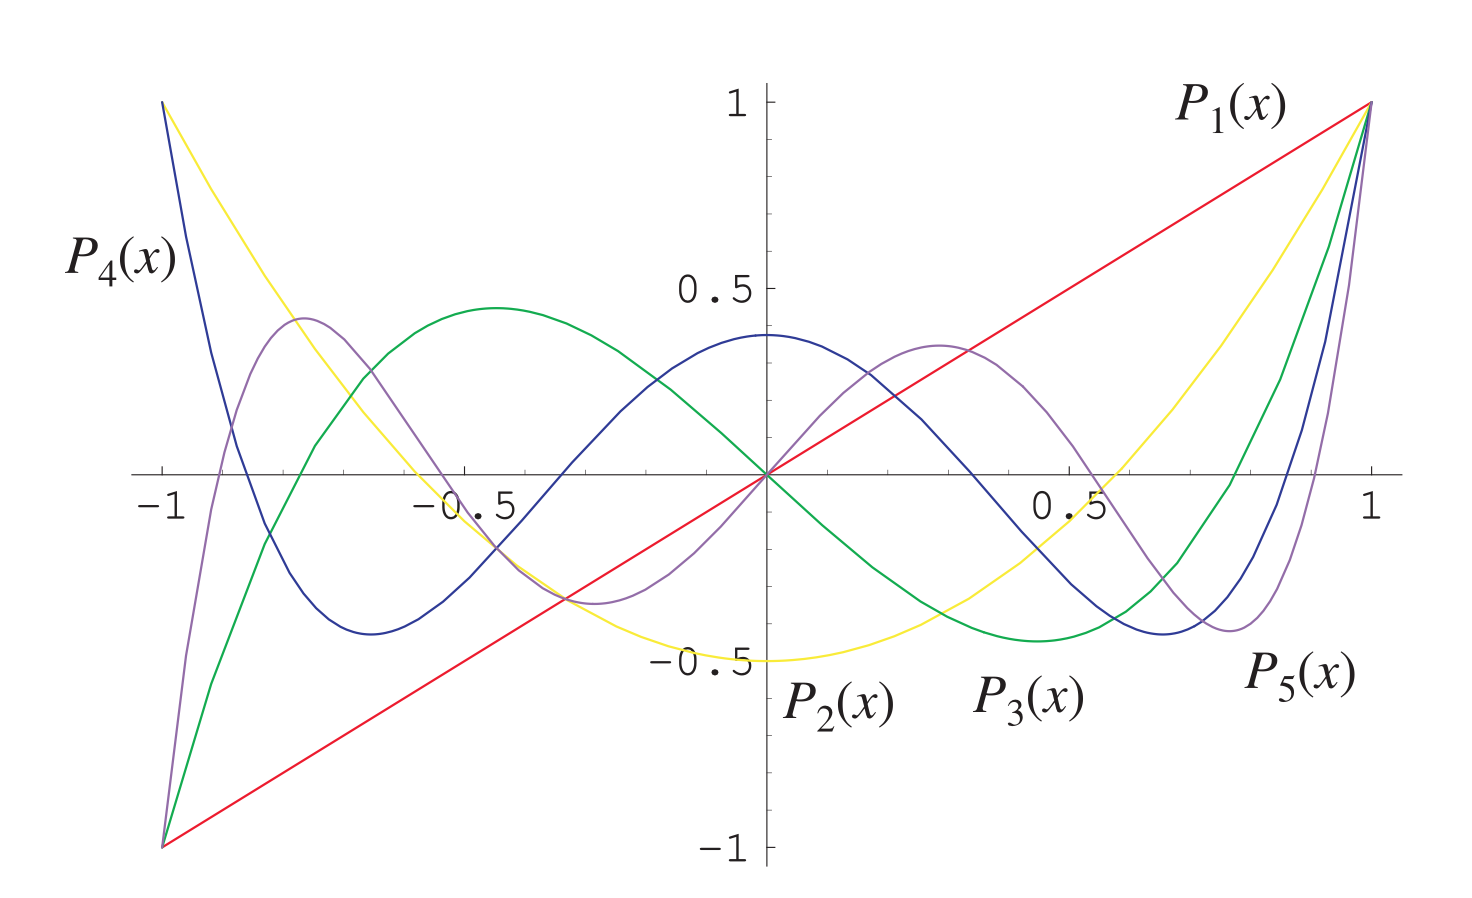
\includegraphics[width=11cm]{figures/LegendrePolynomials.png} 
    \caption{Legendre多项式(注意到奇偶性与$l$一致)} 
    \label{LegendrePolynomials}
\end{figure}

利用$(1-x^2)\mathrm{P}_l''-2x\mathrm{P}_l'+l(l+1)\mathrm{P}_l=0$可以证明
$$\int_x^1\mathrm{P}_k(x)\mathrm{P}_l(x)\mathrm{d}x=\left(1-x^2\right)\frac{\mathrm{P}_k^{\prime}(x)\mathrm{P}_l(x)-\mathrm{P}_l^{\prime}(x)\mathrm{P}_k(x)}{k(k+1)-l(l+1)},\quad k\neq l.$$


\subsubsection{微分表示}

\begin{thm}[Leibniz rule]
    $$
    (uv)^{(n)}=\sum_{k=0}^n\mathrm{C}_n^ku^{(n-k)}n^{(k)}
    $$
\end{thm}

$$\boxed{\mathrm{P}_l(x)=\frac{1}{2^ll!}[(x^2-1)^l]^{(l)}}$$

$$
\begin{aligned}
\mbox{例:}\mathrm{P}_1(x)=&\frac{1}{2}\frac{d}{dx}(x^2-1)=x\\
\mathrm{P}_2(x)=&\frac{1}{8}\frac{d^2}{dx^2}(x^4-2x^2+1)=\frac{1}{2}(3x^2-1)
\end{aligned}
$$

\begin{prf}[$\mathrm{P}_l(x)$满足Legendre方程]
$$$$

设$y=(x^2-1)^l$
$$y'=2lx(x^2-1)^{l-1}\Rightarrow(x^2-1)y'=2lx(x^2-1)^l=2lxy$$

对上式求$l+1$阶导数

$$
(x^2-1)y^{(l+2)}+(l+1)y^{(l+1)}2x+\frac{l(l+1)}{2}y^{(l)}\cdot2=2lxy^{(l+1)}+2l(l+1)y^{(l)}
$$
$$(1-x^2)y^{(l+2)}-2xy^{(l+1)}+l(l+1)y^{(l)}=0$$

因此$y^{(l)}$满足Lengendre方程
\end{prf}

由于我们通常约定$\mathrm{P}_l(1)=1$,因此$\mathrm{P}_l(x)=\frac{1}{y^{(l)}(1)}y^{(l)}(x)$,其中
$$
\begin{aligned}
&y^{(l)}(1)=[(x^2-1)^l]^{(l)}|_{x=1}\\
=&[(x-1)^l(x+1)^l]^{(l)}|_{x=1}\\
=&[(x-1)^l]^{(l)}(x+1)^l|_{x=1}+l[(x-1)^l]^{(l-1)}[(x+1)^l]'|_{x=1}+...\\
=&l!2^l\\
\Rightarrow&\mathrm{P}_l(x)=\frac{1}{2^ll!}[(x-1)^l]^{(l)}
\end{aligned}
$$

\begin{ex}计算:
$$
\int_{-1}^{1}x^k\mathrm{P}_l(x)dx
$$

由$\mathrm{P}_l(x)=(-1)^l\mathrm{P}_l(-x)$可知,$l$为奇数时为奇函数,为偶数时为偶函数;若$k\pm l$为奇数,积分为零,则当$k\pm l$为偶数时
$$\begin{aligned}
&\int_{-1}^{1}x^k\mathrm{P}_l(x)dx\\
=&\frac{1}{2^ll!}\int_{-1}^1x^k[(x^2-1)^l]^{(l)}dx\\
=&\frac{1}{2^ll!}x^k[(x^2-1)^l]^{(l-1)}|_{-1}^1-\frac{1}{2^ll!}\int_{-1}^1(x^k)'[(x^2-1)^l]^{(l-1)}dx\\
=&\dots\\
=&\frac{1}{2^ll!}\int_{-1}^1(x^k)^{(l)}(1-x)^2dx
\end{aligned}$$

$k<l$:$(x^k)^{(l)}=0\Rightarrow 0$

$k\ge l$:$k=l+2n(n\ge0)\Rightarrow$

$$\begin{aligned}
&\int_{-1}^1x^{l+2n}\mathrm{P}_l(x)dx\\
=&\frac{1}{2^ll!}\int_{-1}^1(x^{l+2n})^{(l)}(1-x^2)^ldx\\
=&\frac{1}{2^ll!}\frac{(l+2n)!}{(2n)!}\int_{-1}^1x^{2n}(1-x^2)^ldx\\
\xlongequal{x^2=t}&\frac{1}{2^ll!}\frac{(l+2n)!}{(2n)!}\int_{0}^1t^{n-\frac{1}{2}}(1-t)^ldx\\
=&\frac{1}{2^ll!}\frac{(l+2n)!}{(2n)!}\frac{\Gamma(n+\frac{1}{2})\Gamma(l+1)}{\Gamma(n+l+\frac{3}{2})}\\
=&2^{l+1}\frac{(l+2n)!}{n!}\frac{(l+n)!}{(2l+2n+1)!}
\end{aligned}$$
\begin{rem}
多次利用$\Gamma(x+1)=x\Gamma(x)$
$$
\begin{aligned}
\Gamma(n+l+\tfrac{3}{2})
=&(n+l+\tfrac{1}{2})(n-1+l+\tfrac{1}{2})\dots(1+\tfrac{1}{2})\frac{1}{2}\Gamma(\tfrac{1}{2})
=\frac{1}{2^{2(n+l)+1}}\frac{(2n+2l+1)!}{(n+l)!}\Gamma(\tfrac{1}{2})\\
\Gamma(n+\tfrac{1}{2})=&\frac{1}{2^{2n}n!}\Gamma(\tfrac{1}{2})
\end{aligned}$$


\end{rem}
\begin{dfn}[Beta函数]
    $$B(p,q)=\int_0^1t^{p-1}(1-t)^{q-1}dt=\frac{\Gamma(p)\Gamma(q)}{\Gamma(p+q)}$$
\end{dfn}

\end{ex}

\begin{ex}
    $$I_l=\int_0^1\mathrm{P}_l(x)dx$$

\noindent $l$为偶数时:利用对称性
    $$I_l=I_{2n}=\int_0^1\mathrm{P}_l(x)dx=\frac{1}{2}\int_{-1}^1\mathrm{P}_{2n}(x)dx=0 \quad l=2n(n=1,2,3,\dots):\quad \mathrm{P}_{2n}(x)\mathrm{P}_0(x)\mbox{正交}$$
\noindent $l$为奇数时:
    $$\begin{aligned}
    I_{2n+1}
    =&\frac{1}{2^{2n+1}(2n+1)!}\int_{0}^1[(x^2-1)^{2n+1}]^{(2n+1)}dx\\
    =&\frac{1}{2^{2n+1}(2n+1)!}[(x^2-1)^{2n+1}]^{(2n)}\bigg|_0^1\\
    =&-\frac{1}{2^{2n+1}(2n+1)!}[(x^2-1)^{2n+1}]^{(2n)}\bigg|_{x=0}\\
    =&-\frac{1}{2^{2n+1}(2n+1)!}[\mathrm{C}_{2n+1}^n(x^2)^{(n)}(-1)^{n+1}]^{(2n)}\bigg|_{x=0}\\
    =&(-1)^n\frac{1}{2^{2n+1}(2n+1)!}\frac{(2n+1)!}{(n+1)!n!}(2n)!\\
    =&\boxed{(-1)^n\frac{(2n-1)!!}{(2n+2)!!}}
    \end{aligned}$$
\end{ex}

\subsubsection{广义傅里叶级数}
\noindent \textbf{正交性:}
$$\int_{-1}^1\mathrm{P}_k(x)\mathrm{P}_l(x)dx=0\quad(k\ne l)$$

$x=\cos\theta$
$$\int_0^{\pi}\mathrm{P}_k(\cos\theta)\mathrm{P}_l(\cos\theta)\sin\theta d\theta=0\quad(k\ne l)$$
$$\boxed{||\mathrm{P}_l||^2=\int_{-1}^1[\mathrm{P}_l(x)]^2dx=\frac{2}{2l+1}}$$
利用正交性确定系数:
$$
\begin{aligned}
&[-1,1]:\quad f(x)=\sum_{l=0}^\infty C_l\mathrm{P}_l(x)\qquad &&C_l=\frac{1}{||\mathrm{P}_l||^2}\int_{-1}^1f(x)\mathrm{P}_l(x)dx=\frac{2l+1}{2}\int_{-1}^1f(x)\mathrm{P}_l(x)dx\\
&[0,\pi]:\quad f(\cos\theta)=\sum_{l=0}^\infty C_l\mathrm{P}_l(\cos\theta)\qquad&&C_l=\frac{2l+1}{2}\int_{-1}^1f(\cos\theta)\mathrm{P}_l(\cos\theta)\sin\theta d\theta
\end{aligned}$$


\subsubsection{生成函数(母函数, Generating Function)}
\textbf{生成函数}:$\{a_n\}$的信息翻译为$f(t)$的信息,后者容易处理,可以导出更多信息,然后再翻译为$\{a_n\}$的信息。
\begin{ex}[斐波那契数列的通项公式]递推关系:$a_n=a_{n-1}+a_{n-2}(n\ge2)$

生成函数:$f(t)=a_0+a_1t+a_2t^2+\dots$
$$\begin{aligned}
\sum_{n=2}^\infty a_nt^n=&\sum_{n=2}^\infty(a_{n-1}t^n+a_{n-2}t^n)\\
f(t)-a_0-a_1t=&t[f(t)-a_0]+t^2f(t)\\
\end{aligned}$$
$$\Rightarrow(1-t-t^2)f(t)=a_0+a_1t-a_0t=1$$
$$f(t)=\frac{1}{1-t-t^2}$$

对$f(t)$泰勒展开可得$a_n$
\end{ex}

\begin{nex}[以物理图像证明:北极放置点电荷]
$$
g(x,t)=\sum_{l=0}^\infty \mathrm{P}_l(x)t^l=\frac{1}{\sqrt{1-2xt+t^2}}
$$

设在距原点$r$处放有一个单位点电荷, 取点电荷所在点的方向为$z$轴方向.

这时点电荷在$(r',\theta,\phi)$点的电势 (显然与$\phi$无关) 
$$d=\sqrt{1-2r\cos\theta+r^2}$$
$$u=\frac{1}{d}=\frac{1}{\sqrt{1-2r\cos\theta+r^2}}$$

球内无电荷,电势满足
$$\nabla^2u=\nabla^2\left(\frac{1}{d}\right)=0$$
分离变量法得到$u$的级数解正是$\sum_{l=0}^\infty \mathrm{P}_l(x)t^l$,计算如下:

分离变量$u=R(r)\Theta(\theta)$,得
$$
\begin{cases}
   \frac{1}{ \sin\theta}\frac{d}{d\theta}\left(\frac{1}{\sin\theta}\right)+\lambda\Theta=0\\
   \frac{d}{dr}\left(r^2\frac{dR}{dr}\right)-\lambda R=0
\end{cases}
$$

$\theta$方向:Legendre方程,本征值和本征函数分别为$\lambda_l=l(l+1),\mathrm{P}_l(\cos\theta)$

$r$方向:欧拉方程,变量代换$r=e^t$,
$$
\frac{d^2R(t)}{dt^2}+\frac{dR(t)}{dt}-l(l+1)R(t)=0
$$
$$\begin{aligned}
R=&A_le^{lt}+B_le^{(l+1)t}=A_lr^l+B_l\frac{1}{r^{l+1}}\\
\Rightarrow u=&\frac{1}{d}=\sum_{l=0}^\infty\left(A_lr^l+B_l\frac{1}{r^{l+1}}\right)\mathrm{P}_l(\cos\theta)\quad,r<1\\
=&\sum_{l=0}^\infty A_lr^l\mathrm{P}_l(\cos\theta)
\end{aligned}$$

$\theta=0$时,上式可得$$u=\sum_{l=0}^\infty A_lr^l$$

另一方面,
$$u=\frac{1}{d}=\frac{1}{1-r}=1+r+r^2+r^3+\dots$$

因此$A_l=1$
$$
\frac{1}{d}=\frac{1}{\sqrt{1-2r\cos\theta+r^2}}=\sum_{l=0}^\infty r^l\mathrm{P}_l(\cos\theta)
$$

令$r=t,\cos\theta=x$,得到生成函数
$$\boxed{g(x,t)=\frac{1}{\sqrt{1-2xt+t^2}}=\sum_{l=0}^\infty t^l\mathrm{P}_l(x)\quad|t|<1}$$

$t>1$:
$$
\begin{aligned}
g(x,t)=&\frac{1}{\sqrt{1-2xt+t^2}}=\frac{1}{t}\frac{1}{\sqrt{1-2x\frac{1}{t}+\left(\frac{1}{t}\right)^2}}\\
=&\frac{1}{t}\sum_{l=0}^\infty\left(\frac{1}{l}\right)^l\mathrm{P}_l(x)=\frac{1}{t}\sum_{l=0}^\infty\frac{1}{t^{l+1}}\mathrm{P}_l(\cos\theta)
\end{aligned}$$

\end{nex}
\begin{app}[计算$||\mathrm{P}_l||^2$]
$$[g(x,t)]^2=\frac{1}{1-2xt+t^2}=\left[\sum_{l=0}^\infty t^l\mathrm{P}_l(x)\right]^2$$

两边积分,利用正交性$\int_{-1}^1\mathrm{P}_l\mathrm{P}_kdx=0,l\ne k$
$$\int_{-1}^1\frac{dx}{1-2xt+t^2}=\sum_{l=0}^\infty t^{2l}\int_{-1}^1[\mathrm{P}_l(x)]^2dx$$

对左边进行泰勒展开
$$\frac{1}{2t}\int_{(1-t)^2}^{(1+t)^2}\frac{dy}{y}=\frac{1}{t}\ln\frac{1+t}{1-t}=2\sum_{l=0}^\infty\frac{t^{2l}}{2l+1}$$

得到
$$\int_{-1}^1[\mathrm{P}_l(x)]^2dx=\frac{2}{2l+1}$$

\end{app}

\begin{app}\textbf{递推关系}
\begin{enumerate}
    \item $x\mathrm{P}_l(x)=\frac{l+1}{2l+1}\mathrm{P}_{l+1}(x)+\frac{l}{2l+1}\mathrm{P}_{l-1}(x)\leftarrow g(x,t)$对$t$求导
    \item $\mathrm{P}'_{l+1}(x)+\mathrm{P}'_{l-1}(x)=2xP'_l(x)+\mathrm{P}_l(x)\leftarrow g(x,t)$对$x$求导
    \item $\mathrm{P}'_{l+1}(x)=xP'_l(x)+(l+1)\mathrm{P}_l(x)$
    \item $\mathrm{P}'_{l-1}(x)=xP'_l(x)-l\mathrm{P}_l(x)$
\end{enumerate}
\end{app}

\begin{ex}[地球外部引力场]球外Laplace方程
$$U(r,\theta)=\frac{GM}{R}\left[\frac{R}{r}-\sum_{l=2}^\infty a_l\left(\frac{R}{r}\right)^{l+1}\mathrm{P}_l(\cos\theta)\right]$$
\end{ex}

\subsection{连带Legendre方程}
$$(1-x^2)y''-2xy'+\left(\lambda-\frac{m^2}{1-x^2}\right)y=0\quad(m=1,2,3,...)\quad y(\pm1)<\infty$$
\subsubsection{微分表示}
\noindent 1. 将$y(x)$写成$y(x)=(1-x^{2})^{\frac{m}{2}}v(x)$形式

在$x=1$附近求解$y,t=x-1$
$$-t(t+2)y''-2(t+1)y^{\prime}+\left[\lambda+\frac{m^{2}}{t(t+2)}\right]y=0$$

指标方程:$\rho^2=\frac{m^2}{4}$,得$\rho=\pm\frac{m}{2}$,由于$y$不发散,$\rho=\frac{m}{2}$
$$y=t^{\frac{m}{2}}(a_{0}+a_{1}t+\dots)$$
$$y(x)=(x-1)^{\frac m2}[a_0+a_1(x-1)+\dots]$$

$x=-1$附近求解:$y(x)=(x+1)^{\frac m2}[b_0+b_1(x-1)+\dots]$
$$y(x)=(1-x)^{\frac{m}{2}}(1+x)^{\frac{m}{2}}v(x)=(1-x^{2})^{\frac{m}{2}}v(x)$$

代入原方程:
$$(1-x^{2})^{\frac{m}{2}+1}v''-2(m+1)x(1-x^{2})^{\frac{m}{2}}v'+(1-x^{2})^{\frac{m}{2}}[\lambda-m(m+1)]v=0$$

$v(x)$满足以下方程:
$$(1-x^{2})v''-2(m+1)xv'+[\lambda-m(m+1)]v=0$$

\noindent 2. $v(x)$方程$\leftrightarrow$:Legendre方程

$\mathrm{P}_l(x)$满足Legendre方程:$[(1-x^{2})\mathrm{P}_{l}^{\prime}]^{\prime}+\lambda \mathrm{P}_{l}=0$, $\mathrm{P}_l(\pm1)<\infty$, $\lambda=l(l+1)$

求$m$次导数:
$$[(1-x^{2})\mathrm{P}_{l}']^{(m+1)}+\lambda \mathrm{P}_{l}^{(m)}=0$$
$$(1-x^{2})(\mathrm{P}_{l}^{\prime})^{(m+1)}+(m+1)(\mathrm{P}_{l}^{\prime})^{(m)}(-2x)+\frac{m}{2}(m+1)(\mathrm{P}_{l}^{\prime})^{(m-1)}(-2)+\lambda \mathrm{P}_{l}^{(m)}=0$$
$$(1-x^{2})\mathrm{P}_{l}^{(m+2)}-2(m+1)x\mathrm{P}_{l}^{(m+1)}+[\lambda-m(m+1)]\mathrm{P}_{l}^{(m)}=0$$

$\mathrm{P}_{l}^{(m)}$与$v$满足同一方程,因此$v(x)\propto [\mathrm{P}_{l}(x)]^{(m)}$。习惯性取比例为$(-1)^{m}$
$$v(x)=(-1)^{m}[\mathrm{P}_{l}(x)]^{(m)}$$

\textbf{本征函数:}$m$阶$l$次连带Legendre函数
$$\boxed{y_{l}(x)=\mathrm{P}_{l}^{m}(x)=(1-x^{2})^{\frac{m}{2}}v=(-1)^{m}(1-x^{2})^{\frac{m}{2}}[\mathrm{P}_{l}(x)]^{(m)}}$$

其中,
$$\mathrm{P}_{l}^{m}(x)=\frac{1}{2^{l}l!^{l}}(-1)^{m}(1-x^{2})^{\frac{m}{2}}[(x^{2}-1)^{l}]^{(l+m)}$$

\textbf{本征值:}$\lambda_l=l(l+1),l=m,m+1,m+2,\dots$(当$m>l$时,$\mathrm{P}_{l}^{m}(x)=0$)

$$
\begin{alignedat}{3}
    &\mathrm{P}_0^0=1\quad    &&\mathrm{P}_1^0=x\quad    &&\mathrm{P}_1^1=-(1-x^2)^{\frac{1}{2}}\\
    &\mathrm{P}_2^0=\frac{1}{2}(3x^2-1)\quad&&\mathrm{P}_2^1=-3x(1-x^2)^{\frac{1}{2}}\quad&&\mathrm{P}_2^2=3(1-x^2)
\end{alignedat}
$$

\noindent 在$\theta$变量下:
$$\frac{1}{\sin\theta}\frac{d}{d\theta}\left(\sin\theta\frac{d\Theta}{d\theta}\right)+\left(\lambda-\frac{m^2}{\sin^2\theta}\right)\Theta=0,\quad \Theta(0),\Theta(\pi)<\infty$$

\textbf{本征值:}$\lambda_l=l(l+1),l=m,m+1,m+2,\dots$

\textbf{本征函数:}$\mathrm{P}_l^m(\cos\theta)$

\subsubsection{广义傅立叶级数}
\noindent \textbf{正交性:}
$$\int_{-1}^1\mathrm{P}_k^m(x)\mathrm{P}_l^m(x)dx=0\quad(k\ne l)$$
$$||\mathrm{P}_{l}^{m}||^{2}=\int_{-1}^{1}[\mathrm{P}_{l}^{m}(x)]^{2}dx=\frac{2}{2l+1}\frac{(l+m)!}{(l-m)!}$$

$$\begin{aligned}
&[-1,1]:\quad f(x)=\sum_{l=m}^\infty C_l\mathrm{P}_l^m(x)\qquad &&C_l=\frac{1}{||\mathrm{P}_l^m||^2}\int_{-1}^1f(x)\mathrm{P}_l^m(x)dx\\
&[0,\pi]:\quad f(\cos\theta)=\sum_{l=m}^\infty C_l\mathrm{P}_l^m(\cos\theta)\qquad&&C_l=\frac{1}{||\mathrm{P}_l^m||^2}\int_{-1}^1f(\cos\theta)\mathrm{P}_l(\cos\theta)\sin\theta d\theta
\end{aligned}$$

\subsection{球谐函数}
\label{Spherical Harmonics}
\noindent 球坐标系下的定解问题:
$$\begin{aligned}
    &\nabla^2u=\frac1{r^2}\frac\partial{\partial r}\left(r^2\frac{\partial u}{\partial r}\right)+\frac1{r^2\sin\theta}\frac\partial{\partial\theta}\left(\sin\theta\frac{\partial u}{\partial\theta}\right)+\frac1{r^2\sin^2\theta}\frac{\partial^2u}{\partial\phi^2}=0 \\
    &\left.u\right|_{\theta=0}=\left.u\right|_{\theta=2\pi}<\infty\\
    &\left.u\right|_{\phi=0}=\left.u\right|_{\phi=\pi}<\infty\quad\left.\frac{\partial u}{\partial\phi}\right|_{\phi=0}=\left.\frac{\partial u}{\partial\phi}\right|_{\phi=2\pi} \\
    &\left.u\right|_{r=0}<\infty\left.u\right|_{r=a}=f(\theta,\phi)
    \end{aligned}$$

\noindent 分离变量:$u(r,\theta,\phi)=R(r)S(\theta,\phi)=R(r)\Theta(\theta)\Phi(\phi)$
$$\begin{cases}
    \frac{\mathrm{d}}{\mathrm{d}r}\left[r^2\frac{\mathrm{d}R(r)}{\mathrm{d}r}\right]-\lambda R(r)=0\\
    \frac{1}{\sin\theta}\frac{d}{d\theta}\left(\sin\theta \frac{d\Theta}{d\theta}\right)+\left(\lambda-\frac{\mu}{\sin^2\theta}\right)\Theta=0\\
    \Phi^{\prime\prime}+\mu\Phi=0
\end{cases}$$


\noindent $\phi$方向:$\Phi^{\prime\prime}+\mu\Phi=0$

本征值$\mu_m=m^2,m=0,1,2,\dots$

本征函数$\Phi_0=1\quad\Phi_{m1}=\sin m\phi,\quad\Phi_{m2}=\cos m\phi$

\noindent $\theta$方向:
$$
\frac{1}{\sin\theta}\frac{d}{d\theta}\left(\sin\theta\frac{d\Theta}{d\theta}\right)+\left[\lambda-\frac{\mu}{\sin^2\theta}\right]\Theta=0
$$

本征值:$\lambda_l=l(l+1)\quad(l=0,1,2,...)$

本征函数:$y_l(x)=\mathrm{P}_l^m(x)$
$$S_{lm}(\theta,\phi)=
\begin{cases}
    \mathrm{P}_l^m(\cos\theta)\cos m\phi&m=0,1,\cdots,l\\
    \mathrm{P}_l^m(\cos\theta)\sin m\phi&m=1,2,\cdots,l
\end{cases}$$

\noindent $r$方向:
$$\frac{d}{dr}(r^{2}\frac{dR}{dr})-l(l+1)R=0$$

欧拉方程,变量代换$r=e^t$可得
$$R=C_{l}r^{l}+D_lr^{-(l+1)}=C_{l}r^{l}$$

\noindent 最后得到:
$$\begin{aligned}
    u(r,\theta,\phi)
    &=\boxed{\sum_{l=0}^{\infty}\sum_{m=0}^{l}r^{l}\mathrm{P}_{l}^{m}(\cos\theta)(A_{lm}\cos m\phi+B_{lm}\sin m\phi)}\\
    &=\sum_{l=0}^{\infty}\sum_{m=0}^{l}r^{l}(A_{lm}S_{lm1}+B_{lm}S_{lm2})
\end{aligned}$$

\noindent 正交性:

当且仅当$l=l',m=m',\alpha=\alpha'$时
$$\int_{0}^{\pi}\int_{0}^{2\pi}S_{lm\alpha}(\theta,\phi)S_{l^{\prime}m^{\prime}\alpha^{\prime}}(\theta,\phi)\sin\theta d\theta d\phi\neq0$$
$$\begin{aligned}
    &||S_{lm1}||^{2}=\int_{0}^{\pi}\int_{0}^{2\pi}[\mathrm{P}_{l}^{m}(\cos\theta)]^{2}\cos^{2}m\phi\sin\theta d\theta d\phi=\frac{(l+m)!}{(l-m)!}\frac{2\pi}{2l+1}(1+\delta_{m0})\\
    &||S_{lm2}||^{2}=\int_{0}^{\pi}\int_{0}^{2\pi}[\mathrm{P}_{l}^{m}(\cos\theta)]^{2}\sin^{2}m\phi\sin\theta d\theta d\phi=\frac{(l+m)!}{(l-m)!}\frac{2\pi}{2l+1}
\end{aligned}$$

\noindent 边界条件:
$$u|_{r=a}=f(\theta,\phi)=\sum_{l=0}^{\infty}\sum_{m=0}^{l}a^{l}(A_{lm}S_{lm1}+B_{lm}S_{lm2})$$

$$a^{l}A_{lm}=\frac{1}{||S_{lm1}||^{2}}\int_{0}^{\pi}\int_{0}^{2\pi}f(\theta,\phi)S_{lm1}(\theta,\phi)\sin\theta d\theta d\phi $$
$$a^{l}B_{lm}=\frac{1}{||S_{lm2}||^{2}}\int_{0}^{\pi}\int_{0}^{2\pi}f(\theta,\phi)S_{lm2}(\theta,\phi)\sin\theta d\theta d\phi $$

$f(\theta,\phi)=\sum_{l=0}^{\infty}\sum_{m=0}^{l}(\dots)S_{lm1}+(\dots)S_{lm2}$称为Laplace级数
